%a4paper size
\documentclass[a4paper, 12pt]{article}

\usepackage[margin=1in]{geometry}         % for margin
\usepackage{graphicx}                     % for images
\usepackage[toc,page]{appendix}
\usepackage{fancyhdr}                     %for page number in bottom right
\usepackage{listings}                     % for code blocks
\usepackage{color}                        % for colored code blocks ;)
\usepackage{fixltx2e}                     % for text subscripts
\usepackage[T1]{fontenc}                  % ensures < appear correctly
\usepackage{lmodern}                      % same as above
\usepackage{float}                        % makes figures STAY
\usepackage{minted}                       % used for reading code from file
\usepackage{url}                          % for urls in bibi

\graphicspath{{images/}}

\setlength{\parindent}{0pt}

% code block rules

\definecolor{dkgreen}{rgb}{0,0.6,0}
\definecolor{gray}{rgb}{0.5,0.5,0.5}
\definecolor{mauve}{rgb}{0.58,0,0.82}

\lstset{frame=tb,
  language=python,
  aboveskip=3mm,
  belowskip=3mm,
  showstringspaces=false,
  columns=flexible,
  basicstyle={\small\ttfamily},
  numbers=left,
  numberstyle=\tiny\color{gray},
  keywordstyle=\color{blue},
  commentstyle=\color{dkgreen},
  stringstyle=\color{mauve},
  breaklines=true,
  breakatwhitespace=true,
  tabsize=3
}

%TITLE n such
\title{Real-Time Systems in Video Games}
\author{Joshua Siems}
\date{\today}

%Page numbering in bottom right
\pagestyle{fancy}
%clear header and footer
\fancyhead{}
\fancyfoot{}
%get rid of annoying horizontal line
\renewcommand{\headrulewidth}{0pt}
%do what i HWANT
\fancyfoot[R]{\thepage}

%BEGIN DOCUMENT
\begin{document}

\pagenumbering{gobble}

\maketitle

\pagenumbering{arabic}

\section{Introduction}
    A real-time system is a system that must perform specified tasks within a well-defined time constraint. For example, a microcontroller which must read inputs and produce outputs based on the inputs within a certain amount of time would be known as a real-time system. Another kind of real-time system is a video game. Video games would fall under the soft real-time system category. This means that, unlike a hard real-time system, where a missed deadline results in a fatal error, a soft-real time system still cares about the result of an operation even if the deadline is missed. This paper will discuss how video games are soft real-time systems, and will layout a plan for developing a new kind of priority based task execution feature for video games. Then, the scheduler is tested on a basic video game engine, and the performance benefits are evaluated.

\section{Literature Review}

    \subsection{Video Games as Real-Time Systems}
         The most basic video game must process user inputs, update game variables and update the screen. This must all be completed in a very short amount of time in order to produce the illusion of movement to the user. See Figure \ref{update_cycle} for a simple example of a game loop \cite{sim_env}.
         \\

        \begin{figure}[H]
            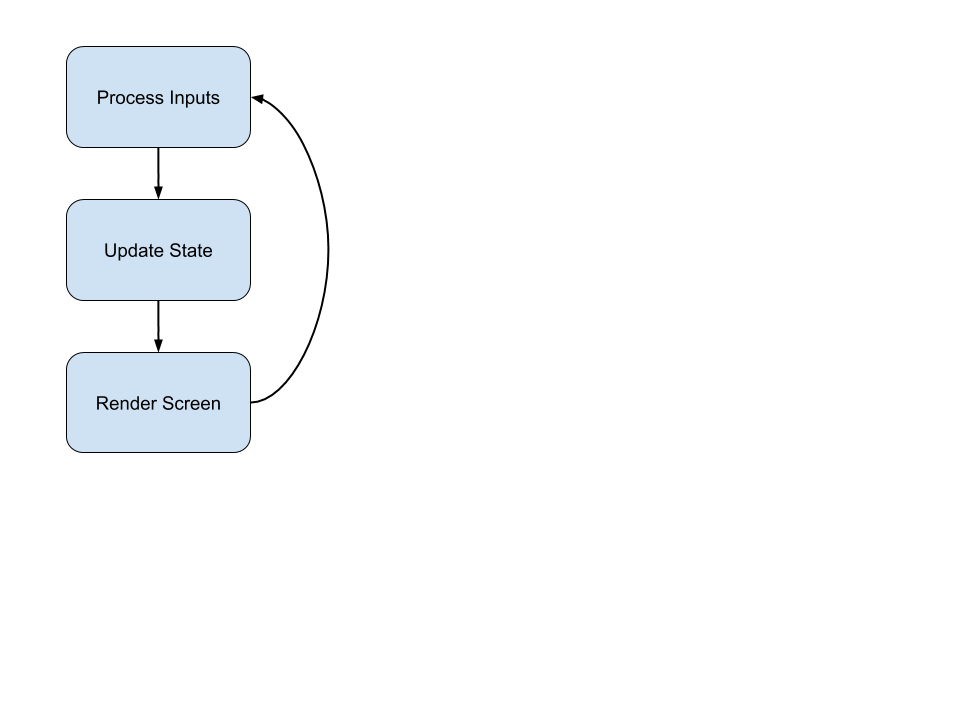
\includegraphics[width=4cm]{game_loop_simple.png}
            \centering
            \caption{Simple game loop.}
            \label{update_cycle}
        \end{figure}

        In order to create this illusion of movement, the game must meet a target frame rate. In the movie world, the industry standard is 24 frames per second. For video games, the targets are much higher. Most games aim to produce at least thirty frames per second, with many more games targeting sixty frames per second \cite{fps}. Some video games are even building in support for even higher frame rates that will allow users to play games on 120Hz or 140Hz monitors. \\

        In this sense, a video game can be thought of as a soft real-time system. A soft real-time system is a real-time system where meeting the deadline is desired, but not required \cite{wiki_rts}. The consequences for missing the deadline in a soft real-time system are miniscule compared to the consequences for missing the deadline in a hard real-time system. For video games, this could be seen as missing the target frame rate for a few frames. The goal is to keep the frame rate close enough to the target so that the user never notices a performance dip. For example, if a game runs at 28 FPS rather than 30 FPS for a few seconds, the user may not even notice. But if a game runs at 15 FPS even for one second, the user will notice the strange delay and the illusion of movement will be ruined. Even then, the game is still playable, and most likely still enjoyable. A video game missing it's deadline is not catastrophic for the user experience, but too many missed deadlines and the player may start to notice \cite{morefps}. \\

    \subsection{Current Video Game Technology}

        Different video games have different requirements when it comes to the game engine being run. A text based adventure game is perhaps the most simple example, requiring almost no deadlines whatsoever \cite{textb}. A text based adventure game will need to read player inputs, and display text to the console. See Figure \ref{text_based_loop}.
        \\

        \begin{figure}[H]
            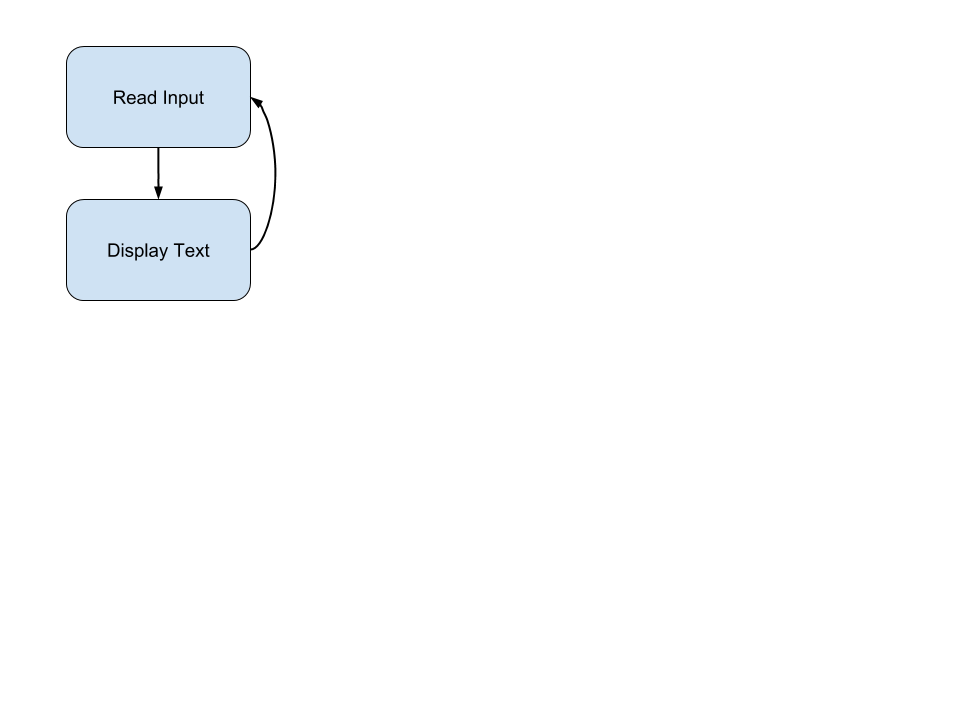
\includegraphics[width=4cm]{text_based_loop.png}
            \centering
            \caption{Text based game loop.}
            \label{text_based_loop}
        \end{figure}

        On the opposite end of the spectrum, a first person shooter may require a much more complex game engine, having to render a 3D world with a sound engine, lighting engine, physics engine, and networking that allows multiple players to play in the same space. All of these components working together creates a very complicated game loop that must fulfill many deadlines \cite{grandmaster}. See Figure \ref{fps_game_loop}.

        \begin{figure}[H]
            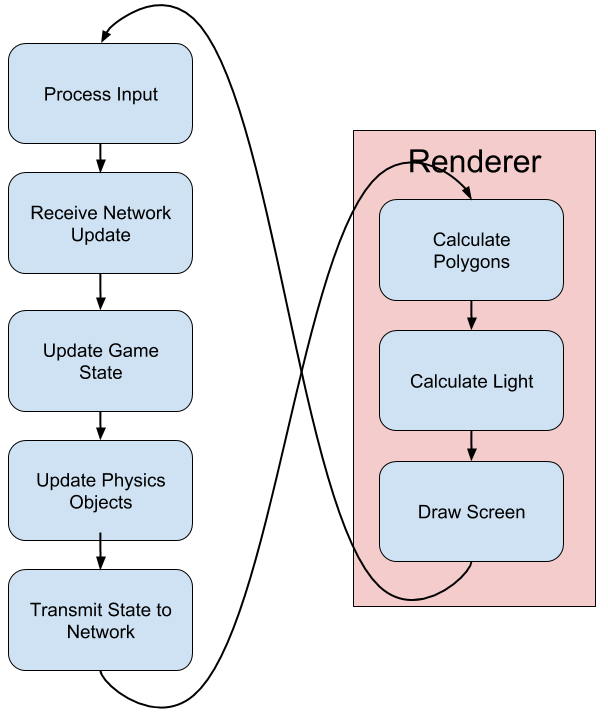
\includegraphics[width=5cm]{fps_loop.png}
            \centering
            \caption{First person shooter game loop \cite{witters}.}
            \label{fps_game_loop}
        \end{figure}

        In order to improve performance, many video games split tasks between many processors. For example, a game engine may split out the rendering task into a process on it's own, and compute all other tasks in a separate thread \cite{cite_gameloop}. This will improve performance because at the same time as objects are being drawn to the screen, the physics engine can update and calculate the next locations for those objects. See Figure \ref{multithread_loop}.

        \begin{figure}[H]
            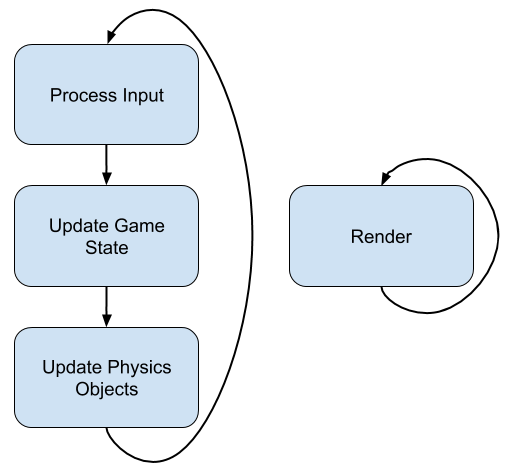
\includegraphics[width=5cm]{multithread_loop.png}
            \centering
            \caption{Multithreaded game loop \cite{rt_gl}.}
            \label{multithread_loop}
        \end{figure}



\section{Methodology}
    \subsection{Goals}

        The goal of this project is to demonstrate the power of a game engine that allows the programmer to dynamically change priorities of tasks. A simple video game will accompany the engine to allow the scheduler to be tested. Experiments will be run on the simple game to see what differences are observed when changing the priorities of tasks. The results from these experiments will be documented and analyzed to determine the success of the project. \\

    \subsection{Pseudocode}
        For the sake of simplicity, this project will use a more basic game loop model that only runs on a single processor. This project will process user inputs, update state variables, update physics objects, and then render the screen using a 2D renderer. This loop is inspired by the Monteiro article \cite{monteiro}. See Figure \ref{my_loop}.

        \begin{figure}[H]
            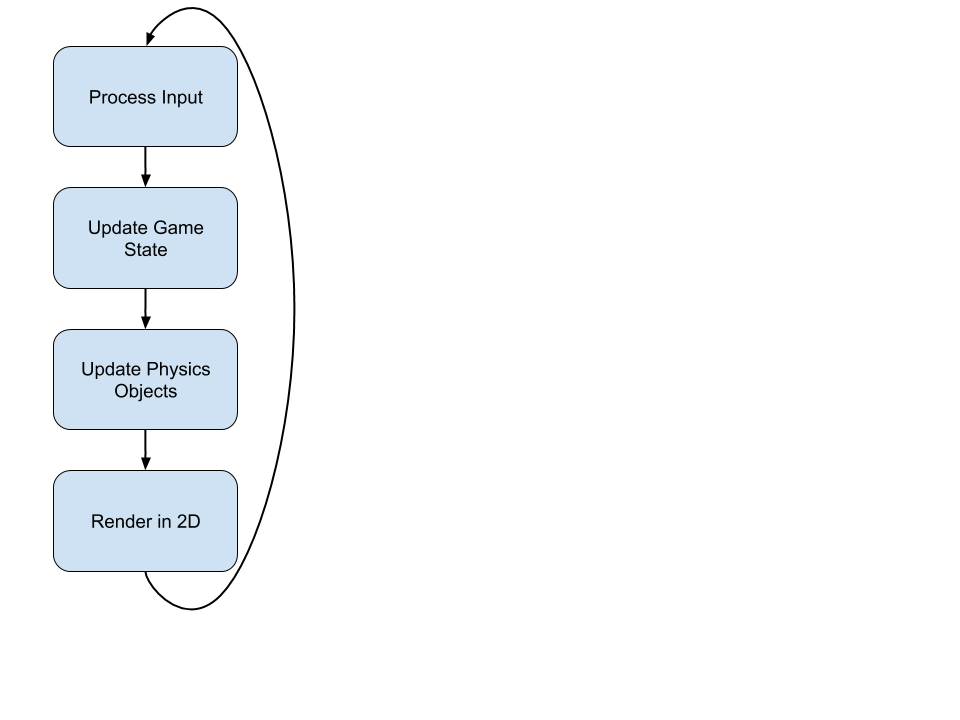
\includegraphics[width=4cm]{my_loop.png}
            \centering
            \caption{Planned game loop for project.}
            \label{my_loop}
        \end{figure}

        The Pseudocode for the program is as follows:

\begin{lstlisting}
main():
    initialize()
    while(playing):
        readInputs()
        updateState()
        updatePhysics()
        drawScreen()

    terminate()
\end{lstlisting}

    \subsection{Scheduler}

        This program will attempt to test a new way of scheduling tasks, one that allows the programmer to change priorities on the fly. The main goal of this scheduler will be to allow the programmer to set priorities of each of the four main loop functions dynamically. For example, if the programmer knows that a certain section requires many physics calculations, he or she can assign the bulk of the run-time to the physics updater. This will in turn reduce the allotted run-time for each of the other processes in the main loop, reducing their accuracy while improving the accuracy of the physics updater.
        \\

        The scheduler will execute the following procedure:
        \begin{enumerate}
            \item{Designate a target frame rate to always meet.}
            \item{Calculate how long each main loop should last based on the given frame rate.}
            \item{Allow the programmer to assign priorities to each process.}
            \item{Allow each process to run for a portion of the loop based on its priority.}
        \end{enumerate}

        For example, if all 4 processes are given a priority of 2, each one would run for 25\% of the time allotted for the main loop. See Figure \ref{even_priority} for an example of this situation. 
        
        \begin{figure}[H]
            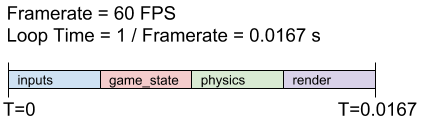
\includegraphics[width=8cm]{even_priority.png}
            \centering
            \caption{Processing distribution with even priority.}
            \label{even_priority}
        \end{figure}

        If updatePhysics() is given a priority of 4, and the others are all 2, updatePhysics() will run for 40\% of the loop while each other function will only run for 20\%. See Figure \ref{phys_priority} for an example of this.

        \begin{figure}[H]
            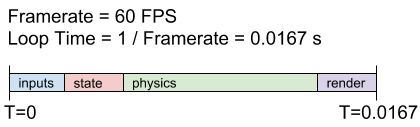
\includegraphics[width=8cm]{phys_priority.png}
            \centering
            \caption{Processing distribution that favors physics calculations}
            \label{phys_priority}
        \end{figure}

    \subsection{Test Environment}

        In order to test the performance benefits of the new scheduler, it was necessary to create a test environment. This test environment will assist in judging the effectiveness of the scheduler. A simple game engine using the pseudocode provided above was created and used as a test environment.
        \\

        The game engine created is very simple when compared to other more modern engines. This was by design, as the simpler the engine was, the easier it would be to judge the performance. The engine can draw circles and rectangles. Circles can either be static or dynamic, while rectangles can only be static. If an object is static, it will never move. If an object is dynamic, it has associated physics variables, such as velocity and restitution. Dynamic objects are updated by the physics updater every game loop.
        \\

        The engine also supports user input. It does this by adding a dynamic circle that follows the users mouse around. This allows the user to interact with the world, and allows for judging the responsiveness of the engine when using the scheduler. The engine will spawn circles at random positions near the top of the screen at a set interval. This interval can be increased or decreased by the user using the up and down arrow keys. The engine can also switch between using the scheduler and not using the scheduler at a press of a button. This was necessary to judge the performance of the scheduler running in the same situation as the engine was running without the scheduler. 
        \\
        
        \begin{figure}[H]
            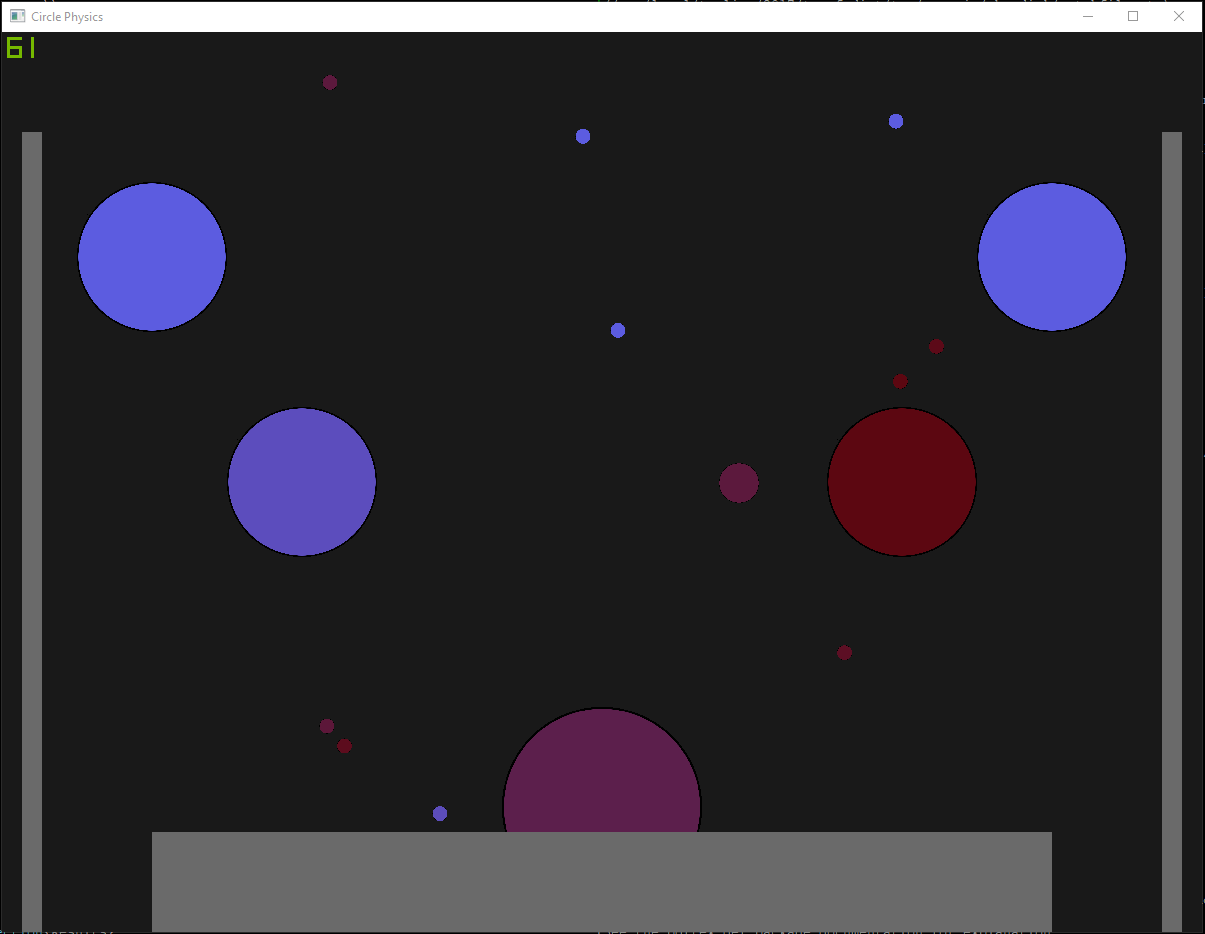
\includegraphics[width=8cm]{engine.png}
            \centering
            \caption{Basic game engine created as a test environment.}
            \label{engine}
        \end{figure}

    \subsection{Testing Procedure}

    The procedure for testing the effectiveness and performance benefits of the scheduler is as follows:
    \begin{enumerate}
        \item{Run the test environment with a low amount of objects. Observe the performance and frame rate of the engine without the scheduler running in this low intensity environment.}
        \item{Press the right arrow key so the engine switches to using the scheduler. Observe the performance and frame rate of the engine with the scheduler in this low intensity environment.}
        \item{Press the right arrow key to turn off the scheduler.}
        \item{Press the up arrow key to increase the spawn rate of the circles. Continue to increase the spawn rate until the system is stressed and the frame rate drops to about ten frames per second.}
        \item{Observe the performance and frame rate of the engine without the scheduler running in this high intensity environment.}
        \item{Press the right arrow key so the engine switches to using the scheduler. Observe the performance and frame rate of the engine with the scheduler in this high intensity environment.}
        \item{Compare the performance and frame rates of the test environment running with and without the scheduler.}
    \end{enumerate}



\section{Results}
    
    When running the engine with no scheduler at a low computation load, everything ran smoothly. The circles appeared to have accurate physics and the circle controlled by the users mouse was responsive. The same is true for running the engine with the scheduler with a low load.
    \\

    The interesting results come from running the engine with a large number of physics calculations. When running the engine with many circles and no scheduler, the entire engine began to slow down. The frames per second dropped down to about ten. The circles appeared to update choppy, and the illusion of movement was ruined. Running the overloaded system with the scheduler is when the interesting results occurred. The circles physics still did not appear to update as fast as desired, but the frame rate was a stable 60 frames per second. This is due to the fact that although the physics process was not able to update the physics variables for every circle every loop, the render process would still draw the circles every loop. Also, a huge difference was noted with the user input process. The responsiveness and accuracy of the circle being controlled by the users mouse was greatly improved compared to when the scheduler was not being used. This is due to the fact that the physics process was given a strict amount of time to update, and the user input process was able to update every loop at the target frame rate. 
    \\

    It is difficult to describe the results of this experiment using only words. It is much easier to see the results in video form. As such, a video presentation of this experiment exists and can be downloaded from: theofficialjosh.com/rts. The most important files created for this project can be viewed in the appendices. All of the code for this project can be viewed at github.com/jsiems/rts\_project.

\section{Conclusion}
    The usefulness of this scheduler can be seen in the results section. As demonstrated in the single use case shown, the scheduler can be used to improve performance of different processes being used by the game engine when other processes are demanding large amounts of resources. In the example given, the user input process was improved even though the physics process was demanding much of the time of the system. 
    \\

    There are many potential use cases of these scheduler. For example, the scheduler could be easily modified to support dynamic assignment of physics calculations based on how far away objects are from the player. This would allow the player to play the game at a high frame rate, and would barely affect gameplay at all as long as the objects far away from the player are less important than the objects close to the player. 
    \\

    The overall usefulness of the scheduler depends on the project it is being implemented in. It is obvious that this scheduler would be very useful in which the accuracy of some processes is less important than the accuracy of others. For example, in the test performed, the accuracy of the physics process was less important than the accuracy of the user input process. By using the scheduler to assign different priorities, the accuracy of the user input process was improved and able to be updated at a more acceptable frame rate and the accuracy of the physics process was sacrificed. If a project requires high accuracy from all processes, it might be a good idea to look for a different solution to getting better frame rates. 
    \\

    This experiment shows how a scheduler can be used to improve the performance of video games. It shows how such a scheduler could work, and demonstrated how the scheduler improved the performance of a simple engine. As video games continue to get larger and more ambitious, and the desire for high quality games increases, video games will have to find more clever ways to improve the performance. This project demonstrates one such way to accomplish just that.

\newpage

% REFERENCES
\section{References}

    \begin{thebibliography}{9}
        \bibitem{sim_env}
            M. Joselli, \textit{A Distributed Architecture for Simulation Environments Based on Game Engine Systems}, 2014. [Online]. Available: \url{https://www.springer.com/cda/content/document/cda_downloaddocument/9783642551307-c2.pdf?SGWID=0-0-45-1463314-p176712314}. [Accessed: 28-Feb-2019].
        \bibitem{fps}
            S. Sarkar, \textit{Why frame rate and resolution matter: A graphics primer}, 2014. [Online]. Available: \url{https://www.polygon.com/2014/6/5/5761780/frame-rate-resolution-graphics-primer-ps4-xbox-one}. [Accessed: 07-May-2019].
        \bibitem{rt_gl}
            L. Valente, \textit{Real Time Game Loop Models for Single-Player Computer Games}, 2005. [Online]. Available: \url{https://pdfs.semanticscholar.org/f401/4a0328b383ee509ed837ff16af96af1168eb.pdf}. [Accessed: 05-March-2019].
        \bibitem{wiki_rts}
            \textit{Real-time computing: Criteria for real-time computing}, 2019. [Online]. Available: \url{https://en.wikipedia.org/wiki/Real-time_computing#Criteria_for_real-time_computing}. [Accessed: 07-May-2019].
        \bibitem{grandmaster}
            \textit{Game Engine part 4}, 2014. [Online]. Available: \url{http://www.grandmaster.nu/blog/?page_id=261}. [Accessed: 05-March-2019].
        \bibitem{morefps}
            M. Klappenbach, \textit{Understanding and Optimizing Video Game Frame Rates}, 2018. [Online]. Available: \url{https://www.lifewire.com/optimizing-video-game-frame-rates-811784}. [Accessed: 05-March-2019].
        \bibitem{cite_gameloop}
            \textit{Game Loop}, n.d. [Online]. Available: \url{http://gameprogrammingpatterns.com/game-loop.html}. [Accessed: 05-March-2019].
        \bibitem{witters}
            K. Witters, \textit{deWiTTERS Game Loop}, 2009. [Online]. Available: \url{http://www.koonsolo.com/news/dewitters-gameloop/}. [Accessed: 05-March-2019].
        \bibitem{monteiro}
            R. Monteiro, \textit{Understanding the Game Main Loop}, 2010. [Online]. Available: \url{http://higherorderfun.com/blog/2010/08/17/understanding-the-game-main-loop/}. [Accessed: 05-March-2019].
        \bibitem{textb}
            D. Cox, \textit{Interactive Fiction: Text Adventures}, 2013. [Online]. Available: \url{https://gamedevelopment.tutsplus.com/articles/interactive-fiction-text-adventures--gamedev-9996}. [Accessed: 05-May-2019].
    \end{thebibliography}

\newpage

\begin{appendices}

\section{main.c}
    \inputminted{c}{../main.c}
    \newpage

\section{phys.h}
    \inputminted{c}{../src/phys.h}
    \newpage

\section{phys.c}
    \inputminted{c}{../src/phys.c}
    \newpage

\end{appendices}

\end{document}







